\documentclass[twocolumn, 10pt,a4j]{jsarticle}
\usepackage{amsmath}
\usepackage[dvipdfmx]{graphicx}
\usepackage{url}
\usepackage{here}
% プリアンブル
\title{\vspace{-2.5cm}再レポート}
\author{1610581 堀田 大地}
\date{2018/5/24}
\begin{document}
\maketitle{}
\vspace{-10zh}
\section{実験項目}
% 実験項目
  \subsection{順序回路}
  % 順序回路
    \subsubsection{Dラッチ回路}
    % Dラッチ回路
      \begin{enumerate}
        \item 考察 \\
        % 考察
          \begin{enumerate}
            \item ストローブ信号がHのとき,Data信号をQに出力していた.
            \item ストローブ信号がLのとき,Data信号をQは出力しなかった.
            \item Data信号が動いているときに,ストローブ信号をHからLにしたとき,
            Data信号の動きに関わらず出力Qの状態は変わらなかった.
            \item 以上の(a)-(b)より,ストローブ信号の機能は,Data信号を
            出力に伝える機能であった.ラッチ機能は,$\overline{Stb}$が
            Lのときに,Data信号をQに伝えないようにするための
            機能であったと考えられた.
          \end{enumerate}
      \end{enumerate}
    \subsubsection{フリップフロップ回路}
    % フリップフロップ回路
        \begin{enumerate}
          \item 実験 \\
          % 実験
            図1に,タイムチャートに従って入力端子を操作したときの出力Q,$\overline{Q}$を示した.
              % 図11
              \begin{figure}[H]
                \begin{center}
                  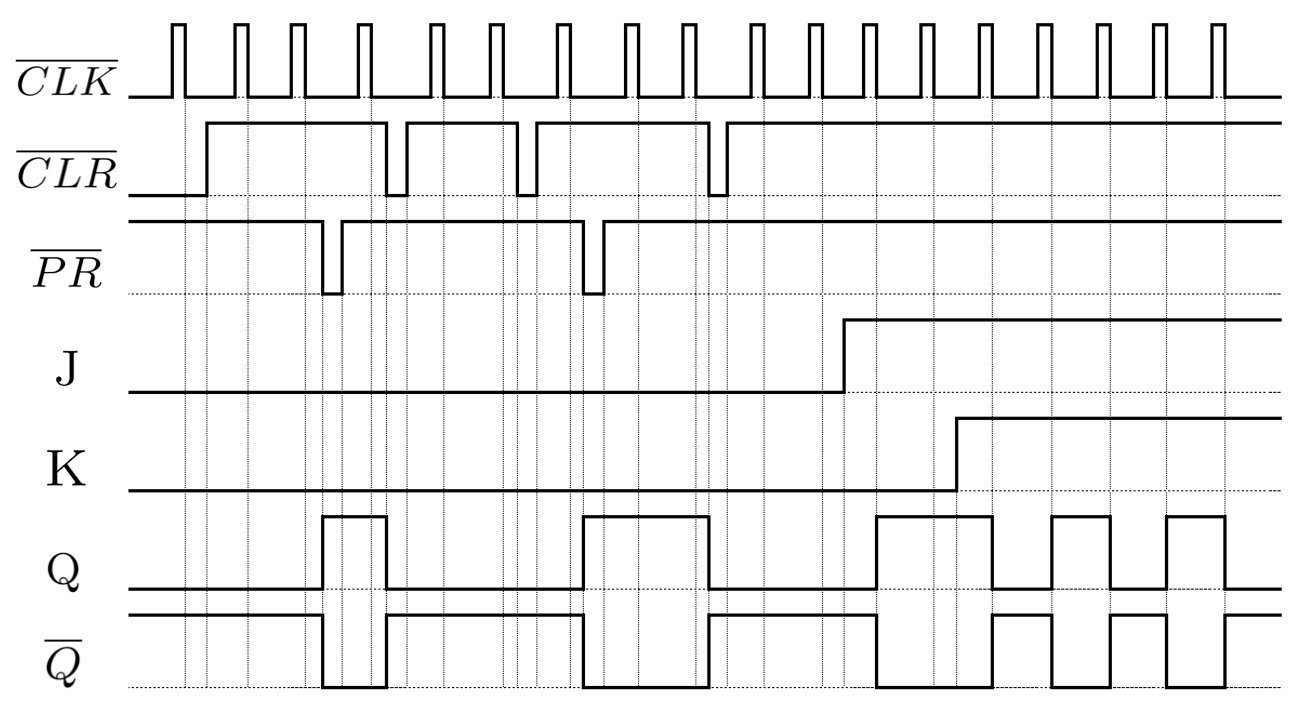
\includegraphics[width=7cm]{../img/junjokairo/jk_flip_flop_time_chart.png}
                  \caption{J-Kフリップフロップ回路のタイムチャート}
                \end{center}
              \end{figure}
          \item 考察 \\
          % 考察
            出力Q,$\overline{Q}$は,$\overline{CLR}$がHで$\overline{PR}$がLになったとき,H,Lになった.
            逆に,$\overline{PR}$がHの状態で$\overline{CLR}$がLになったとき,L,Hになった.
            つまりこの2点から,$\overline{CLR}$はLになると,QをLに,$\overline{Q}$をHに変え,
            $\overline{PR}$はLになると,QをHに,$\overline{Q}$をLに変えていると考えられた.
            $\overline{CLR}$,$\overline{PR}$をHのまま,JをH,KをLの状態にして,
            $\overline{CLK}$をLにすると,QがH,$\overline{Q}$がLになったことより,
            タイムチャート前半の$\overline{PR}$の機能と同じ機能を持つと考えられた.
            また,その状態のままJをL,KをHにして,$\overline{CLK}$をLにすると,
            $\overline{CLR}$の機能と同じ機能を持つと考えられた.
            J,Kを両方Hにすると,$\overline{CLK}$をLにする度,
            前の状態が復元されると考えられた.
        \end{enumerate}
    \subsubsection{Dフリップフロップ回路(74HC74)を用いた$1/2$分周器}
    % Dフリップフロップ回路(74HC74)を用いた$1/2$分周器
      \begin{enumerate}
        \item 実験 \\
        % 実験
          Dフリップフロップのタイムチャートを図2に示した.
          % 図2
            \begin{figure}[H]
              \begin{center}
                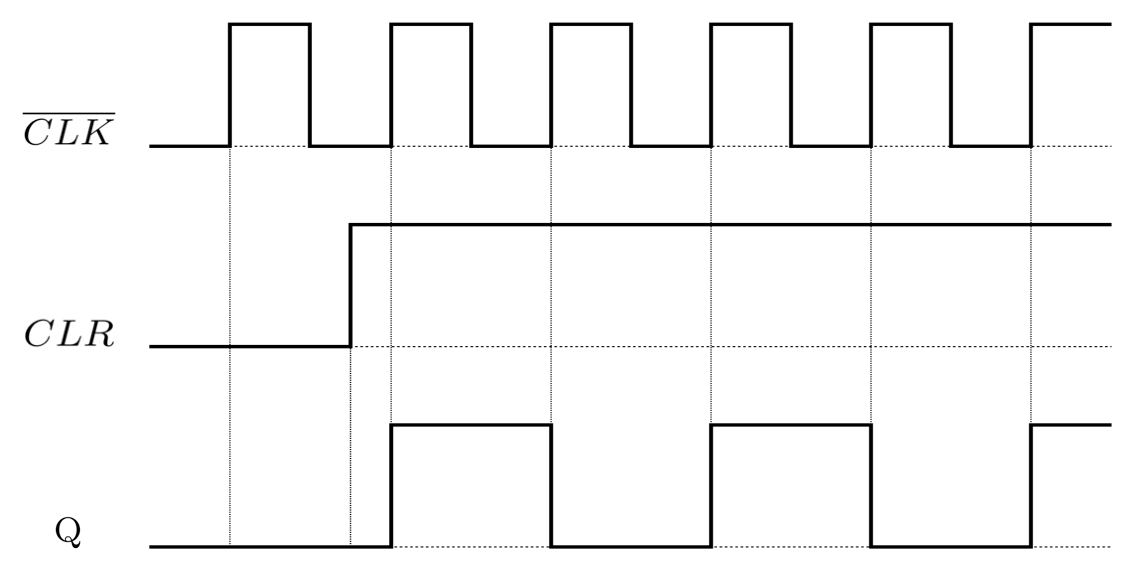
\includegraphics[width=7cm]{../img/junjokairo/d-ff_time_chart.png}
                \caption{Dフリップフロップを用いた$1/2$分周器のタイムチャート}
              \end{center}
            \end{figure}
        \item 考察 \\
        % 考察
          \begin{enumerate}
            \item $\overline{CLR}$がHのときのみ,CLKの立ち上がりの時,出力Qが反転した.
            \item $\overline{CLK}$の2周期分がQの1周期に相当していたので,出力Qは$\overline{CLK}$の倍の周期であった.
            \item 周波数は,周期の逆数なので,出力Qは$\overline{CLK}$の1/2倍の周期であった.
            \item 以上の3点より,分周器の分周機能とは,周波数を分割する機能であると考えられた.

          \end{enumerate}
      \end{enumerate}
  \subsection{カウンタ回路}
  % カウンタ回路
    \subsubsection{非同期16進カウンタ回路}
    % 非同期16進カウンタ回路
      非同期16進カウンタ回路とは,J-Kフリップフロップ回路を4つ用いた回路である.
      タイムチャートを図3に示した.
      % 図3
      \begin{figure}[H]
        \begin{center}
          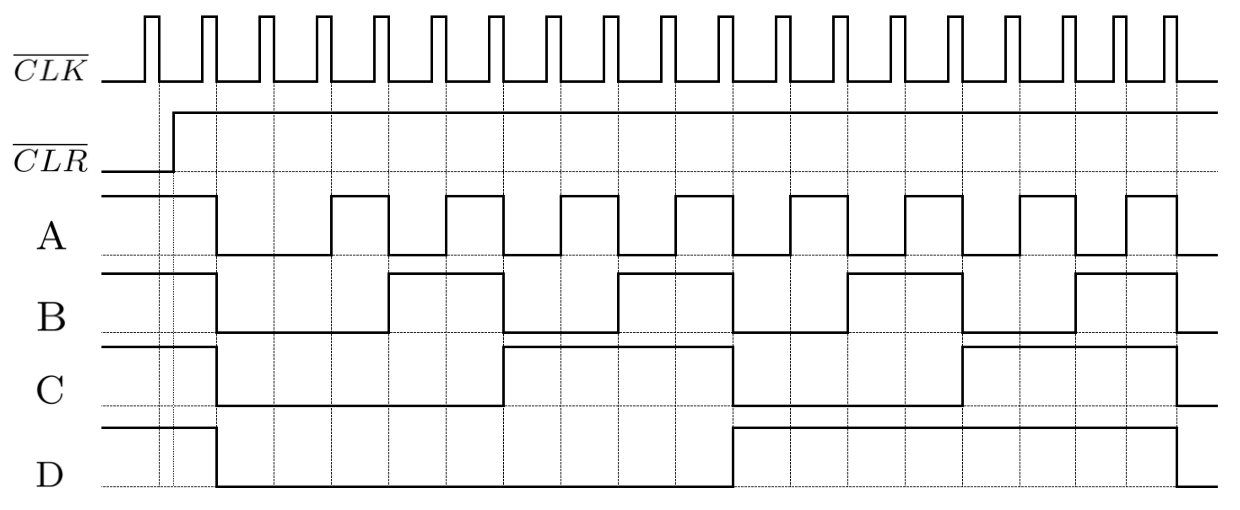
\includegraphics[width=7cm]{../img/junjokairo/hidouki_16shin_dousahyou.png}
          \caption{非同期16進カウンタのタイムチャート}
        \end{center}
      \end{figure}
      \begin{enumerate}
        \item 考察 \\
        % 考察
          \begin{enumerate}
            \item 
              $\overline{CLR }$をLにすると,$\overline{CLK}$に関わらず4つの出力A,B,C,DはHに,NLED1はFになった.
            \item 
              $\overline{CLR}$をHにした後,入力$\overline{CLK}$に立下り信号を入力すると,
              4つの出力は全てLになり,NLED1は0になった
            \item 
              さらに,$\overline{CLK}$をに立下り信号を入力し続けると,
              最初の1回はどの出力もLのままだったが,2回目以降は,
              出力Aは,$\overline{CLK}$が立下がりで毎回,
              出力Bは,2回に1回,
              出力Cは,4回に1回,
              出力Dは,8回に1回,
              NLED1は,16進数表記で1ずつ加算されているように変化していた.
            \item 
              4つの出力をHを1,Lを0とし,
              $2^3D + 2^2C + 2^1B + 2^0A$を計算すると,
              この和がNLED1を10進数に変換したものに等しかった.
            \item 
              入力$\overline{CLK}$と出力Aの周期の間には,
              $1 : 2 = \overline{CLK} : A$の関係があった.
              また,出力AとB,BとC,CとDの間には,$1 : 2 = A : B $,
              $1 : 2 = B : C $,$1 : 2 = C : D $の関係があると考えられた.
              さらに,入力$\overline{CLK}$信号の周期を基準とすると,各周期の大きさの比は$1 : 2 : 4 : 8 :16= \overline{CLK} : A:B:C:D$
              であった.
            \item 
              入力$\overline{CLK}$と出力Aの周波数の間には,周波数は周期の逆数なことを考慮すると,
              $1 : 1/2 = \overline{CLK} : A$の関係があると考えられた.
              また,出力AとB,BとC,CとDの間には,$1 : 1/2 = A : B $,
              $1 : 1/2 = B : C $,$1 : 1/2 = C : D $の関係があると考えられた.
              さらに,入力$\overline{CLK}$信号の周期を基準とすると,各周波数の大きさの比は$1 : 1/2 : 1/4 : 1/8 : 1/16= \overline{CLK} : A:B:C:D$
              であった.
          \end{enumerate}
      \end{enumerate}
      
      

  
\end{document}